% Chapter Template

\chapter{Results - Sliding Puzzle} % Main chapter title

\label{sec:ResultsSP} % Change X to a consecutive number; for referencing this chapter elsewhere, use \ref{ChapterX}

%----------------------------------------------------------------------------------------
%	SECTION 1
%----------------------------------------------------------------------------------------

\section{Low dimension}

As mentioned in chapter \ref{sec:Puzzles}, the state space cardinality for the SP grows very quickly with n and m. Here are the only dimensions which have less than 239.5 millions states. Note I am also only considering n $\leq$ m since (p, q) can always be solved if we know how to solve (q, p):
\\
\\
\begin{center}
\begin{tabular}{l*{6}{c}r}
n              & m & 2 & 3 & 4 & 5\\
\hline
2              &   & 12 & 360 & 20,160 & 1,814,400 \\
3              &   &   & 181,440 &  &    \\
\end{tabular}
\end{center}
In this section, I will discuss learning the value function of these 5 puzzles \textbf{exactly}.
In order to do so, one can simply use rubiks.scripts.learner, setting up the PerfectLearner with A* and manhattan heuristic, or instantiate directly a PerfectLearner as have seen in section \ref{PLSS}
I obtained the following God numbers for these puzzles:
\begin{center}
\begin{tabular}{l*{6}{c}r}
n              & m & 2 & 3 & 4 & 5\\
\hline
2              &   & 6 & 21 & 36 &  \\
3              &   &   & 31 &  &    \\
\end{tabular}
\end{center}
and the most difficult puzzles (requiring a number of steps equal to their respective God number to solves):
\\
\\
\underline{Most difficult 2x2 (6 moves)}:
\begin{center}
\begin{three}
\setrow{2}{,3}
\setrow{1}{2,1}
\end{three}
\end{center}
\underline{Most difficult 2x3 (21 moves)}:
\begin{center}
\begin{five}
\setrow{2}{4,5,}
\setrow{1}{1,2,3}
\end{five}
\end{center}
\underline{Most difficult 2x4 (36 moves)}:
\begin{center}
\begin{seven}
\setrow{2}{,7,2,1}
\setrow{1}{4,3,6,5}
\end{seven}
\end{center}
\underline{Most difficult 2x5 (47 moves) .... TBD }:
\begin{center}
\begin{nine}
\setrow{2}{,2,7,4,1}
\setrow{1}{5,8,3,9,6}
\end{nine}
\end{center}
\underline{Most difficult 3x3 (31 moves)}:
\begin{center}
\begin{eight}
\setrow{3}{8,6,7}
\setrow{2}{2,5,4}
\setrow{1}{3,,1}
\end{eight}
\end{center}



%-----------------------------------
%	SECTION 2
%-----------------------------------
\section{Intermediary case - 3x3}
\label{S33}
As seen above, we have actually been able to solve the 3 by 3 case perfectly, since it only has 181,440 possible configurations. Its God number is only 31, which definitely makes it manageable. However, this is already an intermediary size, large enough to make trying deep reinforcement learning meaningful.



\begin{landscape}
\begin{figure}[H]
\centering
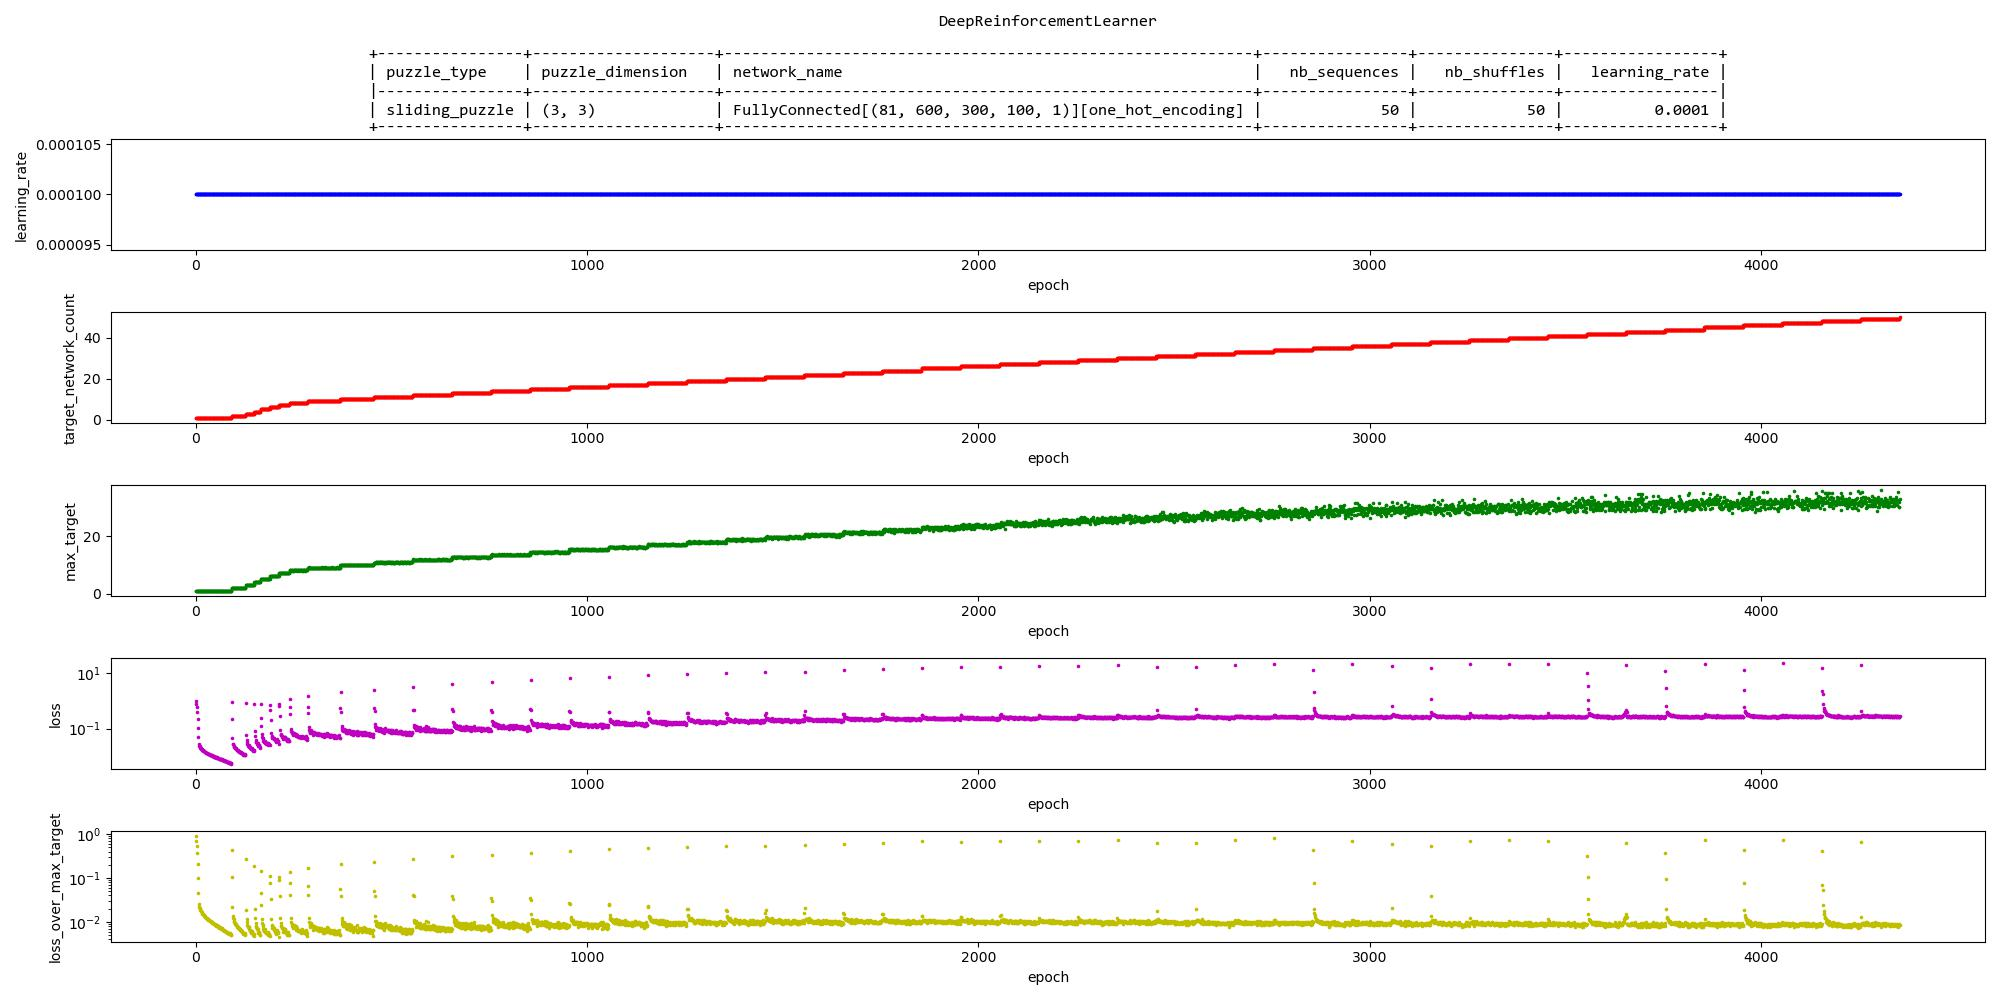
\includegraphics[scale=0.5]{./Figures/33SPDeepReinforcementLearning.jpeg}
%\decoRule
\caption[Codebase]{Code base}
\label{fig:Codebase}
\end{figure}
\end{landscape}


\begin{landscape}
\begin{figure}[H]
\centering
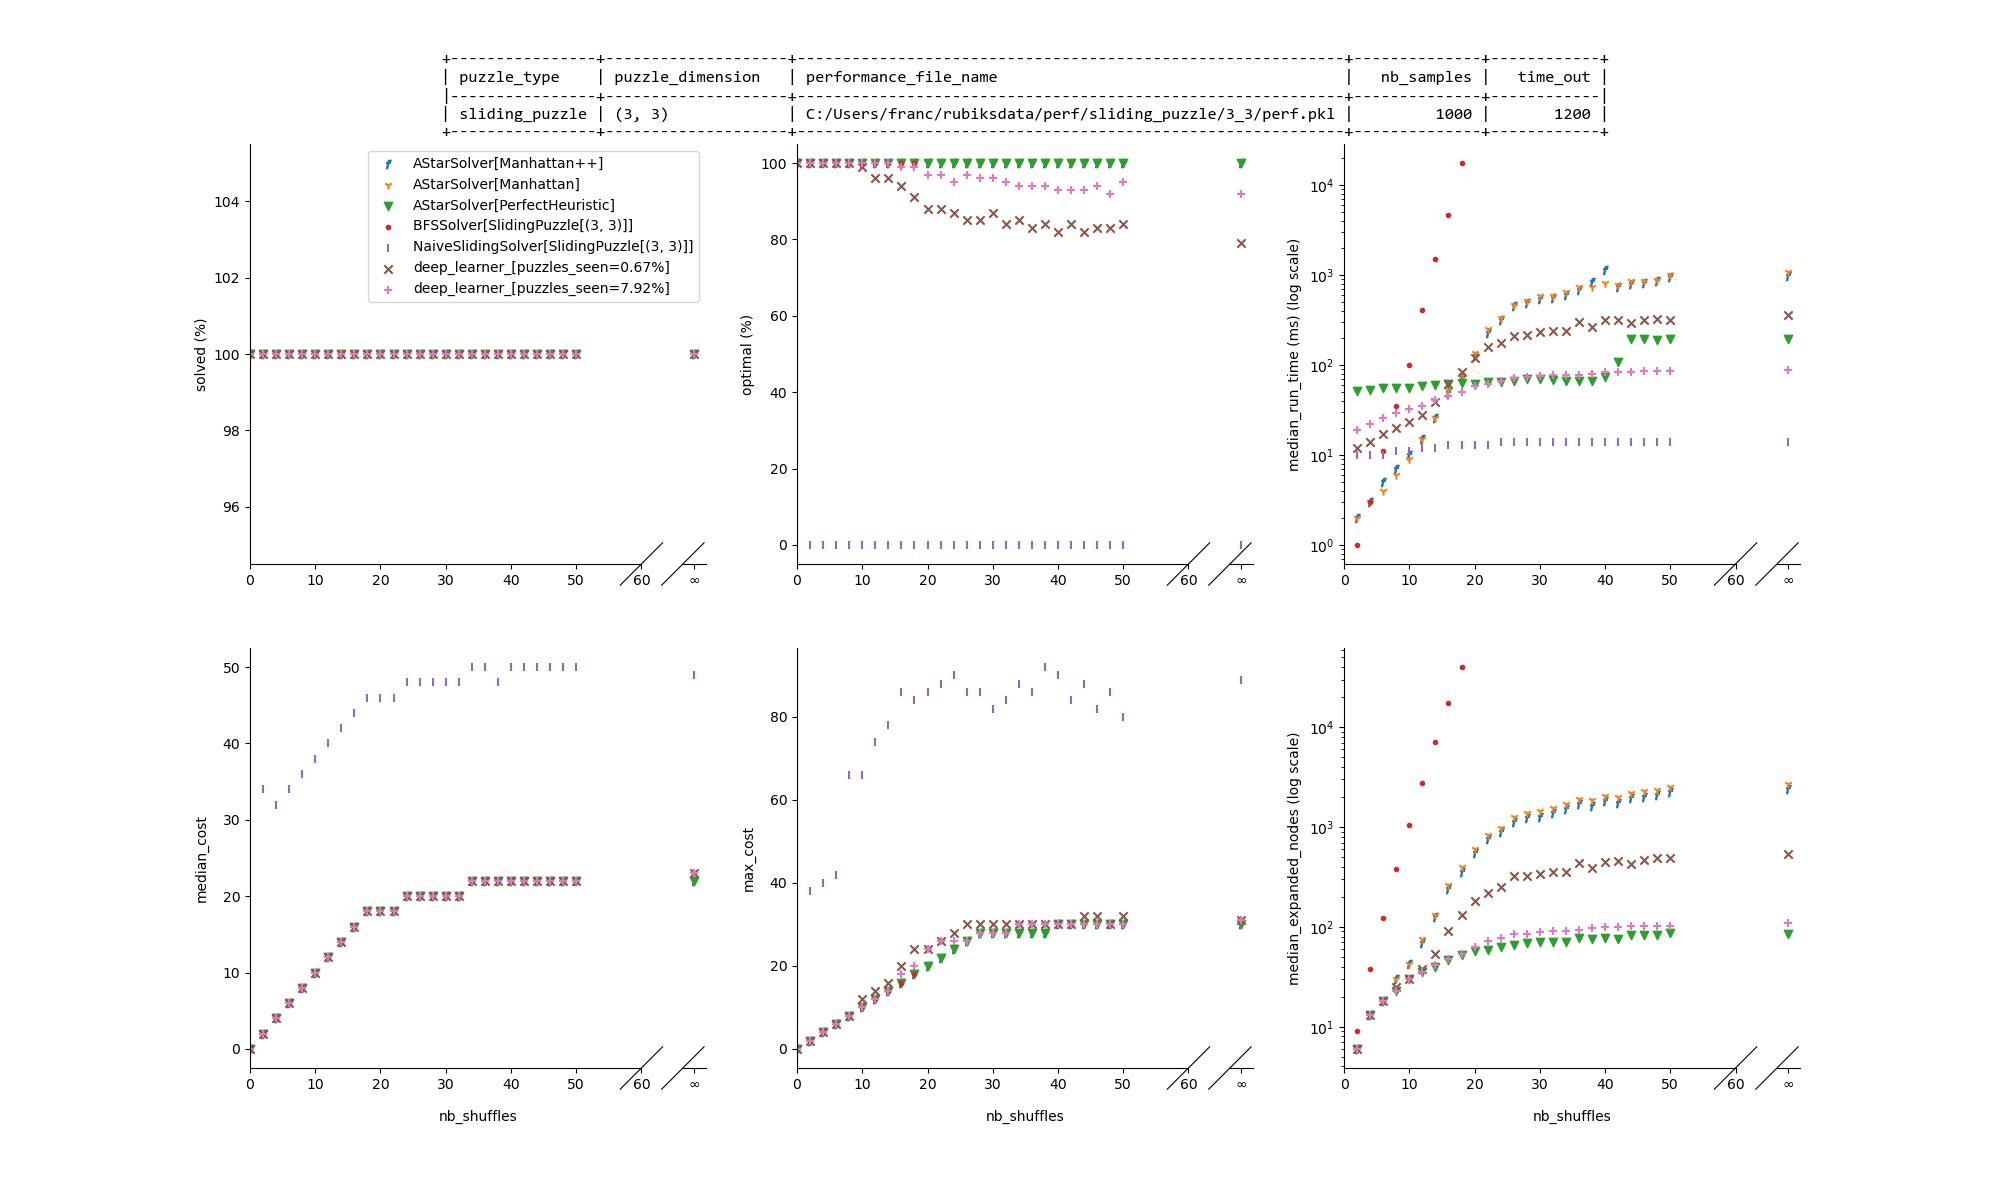
\includegraphics[scale=0.5]{./Figures/33SPPerformance.jpeg}
%\decoRule
\caption[Codebase]{Code base}
\label{fig:Codebase}
\end{figure}
\end{landscape}


%-----------------------------------
%	SECTION 3
%-----------------------------------
\section{3x4}

blabla

%-----------------------------------
%	SECTION 4
%-----------------------------------

\section{4x4}

blabla
